\documentclass[]{article}
\usepackage{lmodern}
\usepackage{amssymb,amsmath}
\usepackage{ifxetex,ifluatex}
\usepackage{fixltx2e} % provides \textsubscript
\ifnum 0\ifxetex 1\fi\ifluatex 1\fi=0 % if pdftex
  \usepackage[T1]{fontenc}
  \usepackage[utf8]{inputenc}
\else % if luatex or xelatex
  \ifxetex
    \usepackage{mathspec}
  \else
    \usepackage{fontspec}
  \fi
  \defaultfontfeatures{Ligatures=TeX,Scale=MatchLowercase}
\fi
% use upquote if available, for straight quotes in verbatim environments
\IfFileExists{upquote.sty}{\usepackage{upquote}}{}
% use microtype if available
\IfFileExists{microtype.sty}{%
\usepackage{microtype}
\UseMicrotypeSet[protrusion]{basicmath} % disable protrusion for tt fonts
}{}
\usepackage[margin=1in]{geometry}
\usepackage{hyperref}
\hypersetup{unicode=true,
            pdftitle={darwin\_revised},
            pdfauthor={GG},
            pdfborder={0 0 0},
            breaklinks=true}
\urlstyle{same}  % don't use monospace font for urls
\usepackage{color}
\usepackage{fancyvrb}
\newcommand{\VerbBar}{|}
\newcommand{\VERB}{\Verb[commandchars=\\\{\}]}
\DefineVerbatimEnvironment{Highlighting}{Verbatim}{commandchars=\\\{\}}
% Add ',fontsize=\small' for more characters per line
\usepackage{framed}
\definecolor{shadecolor}{RGB}{248,248,248}
\newenvironment{Shaded}{\begin{snugshade}}{\end{snugshade}}
\newcommand{\KeywordTok}[1]{\textcolor[rgb]{0.13,0.29,0.53}{\textbf{#1}}}
\newcommand{\DataTypeTok}[1]{\textcolor[rgb]{0.13,0.29,0.53}{#1}}
\newcommand{\DecValTok}[1]{\textcolor[rgb]{0.00,0.00,0.81}{#1}}
\newcommand{\BaseNTok}[1]{\textcolor[rgb]{0.00,0.00,0.81}{#1}}
\newcommand{\FloatTok}[1]{\textcolor[rgb]{0.00,0.00,0.81}{#1}}
\newcommand{\ConstantTok}[1]{\textcolor[rgb]{0.00,0.00,0.00}{#1}}
\newcommand{\CharTok}[1]{\textcolor[rgb]{0.31,0.60,0.02}{#1}}
\newcommand{\SpecialCharTok}[1]{\textcolor[rgb]{0.00,0.00,0.00}{#1}}
\newcommand{\StringTok}[1]{\textcolor[rgb]{0.31,0.60,0.02}{#1}}
\newcommand{\VerbatimStringTok}[1]{\textcolor[rgb]{0.31,0.60,0.02}{#1}}
\newcommand{\SpecialStringTok}[1]{\textcolor[rgb]{0.31,0.60,0.02}{#1}}
\newcommand{\ImportTok}[1]{#1}
\newcommand{\CommentTok}[1]{\textcolor[rgb]{0.56,0.35,0.01}{\textit{#1}}}
\newcommand{\DocumentationTok}[1]{\textcolor[rgb]{0.56,0.35,0.01}{\textbf{\textit{#1}}}}
\newcommand{\AnnotationTok}[1]{\textcolor[rgb]{0.56,0.35,0.01}{\textbf{\textit{#1}}}}
\newcommand{\CommentVarTok}[1]{\textcolor[rgb]{0.56,0.35,0.01}{\textbf{\textit{#1}}}}
\newcommand{\OtherTok}[1]{\textcolor[rgb]{0.56,0.35,0.01}{#1}}
\newcommand{\FunctionTok}[1]{\textcolor[rgb]{0.00,0.00,0.00}{#1}}
\newcommand{\VariableTok}[1]{\textcolor[rgb]{0.00,0.00,0.00}{#1}}
\newcommand{\ControlFlowTok}[1]{\textcolor[rgb]{0.13,0.29,0.53}{\textbf{#1}}}
\newcommand{\OperatorTok}[1]{\textcolor[rgb]{0.81,0.36,0.00}{\textbf{#1}}}
\newcommand{\BuiltInTok}[1]{#1}
\newcommand{\ExtensionTok}[1]{#1}
\newcommand{\PreprocessorTok}[1]{\textcolor[rgb]{0.56,0.35,0.01}{\textit{#1}}}
\newcommand{\AttributeTok}[1]{\textcolor[rgb]{0.77,0.63,0.00}{#1}}
\newcommand{\RegionMarkerTok}[1]{#1}
\newcommand{\InformationTok}[1]{\textcolor[rgb]{0.56,0.35,0.01}{\textbf{\textit{#1}}}}
\newcommand{\WarningTok}[1]{\textcolor[rgb]{0.56,0.35,0.01}{\textbf{\textit{#1}}}}
\newcommand{\AlertTok}[1]{\textcolor[rgb]{0.94,0.16,0.16}{#1}}
\newcommand{\ErrorTok}[1]{\textcolor[rgb]{0.64,0.00,0.00}{\textbf{#1}}}
\newcommand{\NormalTok}[1]{#1}
\usepackage{graphicx,grffile}
\makeatletter
\def\maxwidth{\ifdim\Gin@nat@width>\linewidth\linewidth\else\Gin@nat@width\fi}
\def\maxheight{\ifdim\Gin@nat@height>\textheight\textheight\else\Gin@nat@height\fi}
\makeatother
% Scale images if necessary, so that they will not overflow the page
% margins by default, and it is still possible to overwrite the defaults
% using explicit options in \includegraphics[width, height, ...]{}
\setkeys{Gin}{width=\maxwidth,height=\maxheight,keepaspectratio}
\IfFileExists{parskip.sty}{%
\usepackage{parskip}
}{% else
\setlength{\parindent}{0pt}
\setlength{\parskip}{6pt plus 2pt minus 1pt}
}
\setlength{\emergencystretch}{3em}  % prevent overfull lines
\providecommand{\tightlist}{%
  \setlength{\itemsep}{0pt}\setlength{\parskip}{0pt}}
\setcounter{secnumdepth}{0}
% Redefines (sub)paragraphs to behave more like sections
\ifx\paragraph\undefined\else
\let\oldparagraph\paragraph
\renewcommand{\paragraph}[1]{\oldparagraph{#1}\mbox{}}
\fi
\ifx\subparagraph\undefined\else
\let\oldsubparagraph\subparagraph
\renewcommand{\subparagraph}[1]{\oldsubparagraph{#1}\mbox{}}
\fi

%%% Use protect on footnotes to avoid problems with footnotes in titles
\let\rmarkdownfootnote\footnote%
\def\footnote{\protect\rmarkdownfootnote}

%%% Change title format to be more compact
\usepackage{titling}

% Create subtitle command for use in maketitle
\newcommand{\subtitle}[1]{
  \posttitle{
    \begin{center}\large#1\end{center}
    }
}

\setlength{\droptitle}{-2em}
  \title{darwin\_revised}
  \pretitle{\vspace{\droptitle}\centering\huge}
  \posttitle{\par}
  \author{GG}
  \preauthor{\centering\large\emph}
  \postauthor{\par}
  \predate{\centering\large\emph}
  \postdate{\par}
  \date{12/17/2018}


\begin{document}
\maketitle

\subsection{R Markdown}\label{r-markdown}

\begin{Shaded}
\begin{Highlighting}[]
\KeywordTok{library}\NormalTok{(ggplot2)}
\KeywordTok{library}\NormalTok{(tidyverse)}
\end{Highlighting}
\end{Shaded}

\begin{verbatim}
## -- Attaching packages --------------------------------------- tidyverse 1.2.1 --
\end{verbatim}

\begin{verbatim}
## √ tibble  1.4.2     √ purrr   0.2.4
## √ tidyr   0.8.0     √ dplyr   0.7.4
## √ readr   1.1.1     √ stringr 1.3.0
## √ tibble  1.4.2     √ forcats 0.3.0
\end{verbatim}

\begin{verbatim}
## -- Conflicts ------------------------------------------ tidyverse_conflicts() --
## x dplyr::filter() masks stats::filter()
## x dplyr::lag()    masks stats::lag()
\end{verbatim}

\begin{Shaded}
\begin{Highlighting}[]
\KeywordTok{library}\NormalTok{(readxl)}
\KeywordTok{library}\NormalTok{(janitor)}
\KeywordTok{library}\NormalTok{(dbplyr)}
\end{Highlighting}
\end{Shaded}

\begin{verbatim}
## 
## Attaching package: 'dbplyr'
\end{verbatim}

\begin{verbatim}
## The following objects are masked from 'package:dplyr':
## 
##     ident, sql
\end{verbatim}

\begin{Shaded}
\begin{Highlighting}[]
\NormalTok{darwin <-}\StringTok{ }\KeywordTok{read_csv}\NormalTok{(}\StringTok{"~/Documents/darwin_stats2.csv"}\NormalTok{)}
\end{Highlighting}
\end{Shaded}

\begin{verbatim}
## Parsed with column specification:
## cols(
##   lionfish_den = col_integer(),
##   fish_div = col_double(),
##   fish_den = col_double(),
##   fish_bio = col_double(),
##   temp = col_double(),
##   c_bda = col_double(),
##   c_enchry = col_double(),
##   p_furc = col_double()
## )
\end{verbatim}

\begin{Shaded}
\begin{Highlighting}[]
\KeywordTok{library}\NormalTok{(vegan)}
\end{Highlighting}
\end{Shaded}

\begin{verbatim}
## Warning: package 'vegan' was built under R version 3.4.4
\end{verbatim}

\begin{verbatim}
## Loading required package: permute
\end{verbatim}

\begin{verbatim}
## Loading required package: lattice
\end{verbatim}

\begin{verbatim}
## This is vegan 2.5-1
\end{verbatim}

Visualizing the GLM resutls with a PCA analysis

\begin{Shaded}
\begin{Highlighting}[]
\CommentTok{# remove unwanted variables }
\NormalTok{darwin.pca <-}\StringTok{ }\NormalTok{darwin[, }\DecValTok{2}\OperatorTok{:}\DecValTok{8}\NormalTok{]}
\NormalTok{darwin.pca[}\DecValTok{6}\NormalTok{] =}\StringTok{ }\OtherTok{NULL}
\NormalTok{darwin.pca[}\DecValTok{5}\NormalTok{] =}\StringTok{ }\OtherTok{NULL}
\NormalTok{darwin.den <-}\StringTok{ }\NormalTok{(darwin[, }\DecValTok{1}\NormalTok{] }\OperatorTok{+}\DecValTok{1}\NormalTok{)}
 
\CommentTok{# apply PCA - scale. = TRUE is highly }
\CommentTok{# advisable, but default is FALSE. }
\NormalTok{pca <-}\StringTok{ }\KeywordTok{prcomp}\NormalTok{(darwin.pca,}
                 \DataTypeTok{center =} \OtherTok{TRUE}\NormalTok{,}
                 \DataTypeTok{scale. =} \OtherTok{TRUE}\NormalTok{) }
\end{Highlighting}
\end{Shaded}

\begin{Shaded}
\begin{Highlighting}[]
\CommentTok{# print method}
\KeywordTok{print}\NormalTok{(pca)}
\end{Highlighting}
\end{Shaded}

\begin{verbatim}
## Standard deviations (1, .., p=5):
## [1] 1.6353447 1.0393839 0.7782248 0.6744062 0.4299666
## 
## Rotation (n x k) = (5 x 5):
##                   PC1         PC2        PC3         PC4         PC5
## fish_div -0.003413205 -0.91211057 -0.4080347  0.01744689  0.03529841
## fish_den  0.548495322 -0.10675208  0.3076731  0.24452022  0.73027666
## fish_bio  0.521156727  0.08609343 -0.2128905  0.64775332 -0.50604039
## temp     -0.439450793 -0.29667886  0.6738480  0.48878935 -0.16086802
## p_furc    0.484169287 -0.24744267  0.4893378 -0.53047722 -0.42836272
\end{verbatim}

In order to create the biplot we need devtools and ggbiplot available
from CRAN and github

\begin{Shaded}
\begin{Highlighting}[]
\KeywordTok{library}\NormalTok{(devtools)}
\end{Highlighting}
\end{Shaded}

\begin{verbatim}
## Warning: package 'devtools' was built under R version 3.4.4
\end{verbatim}

\begin{verbatim}
## 
## Attaching package: 'devtools'
\end{verbatim}

\begin{verbatim}
## The following object is masked from 'package:permute':
## 
##     check
\end{verbatim}

\begin{Shaded}
\begin{Highlighting}[]
\KeywordTok{library}\NormalTok{(ggbiplot)}
\end{Highlighting}
\end{Shaded}

\begin{verbatim}
## Loading required package: plyr
\end{verbatim}

\begin{verbatim}
## -------------------------------------------------------------------------
\end{verbatim}

\begin{verbatim}
## You have loaded plyr after dplyr - this is likely to cause problems.
## If you need functions from both plyr and dplyr, please load plyr first, then dplyr:
## library(plyr); library(dplyr)
\end{verbatim}

\begin{verbatim}
## -------------------------------------------------------------------------
\end{verbatim}

\begin{verbatim}
## 
## Attaching package: 'plyr'
\end{verbatim}

\begin{verbatim}
## The following objects are masked from 'package:dplyr':
## 
##     arrange, count, desc, failwith, id, mutate, rename, summarise,
##     summarize
\end{verbatim}

\begin{verbatim}
## The following object is masked from 'package:purrr':
## 
##     compact
\end{verbatim}

\begin{verbatim}
## Loading required package: scales
\end{verbatim}

\begin{verbatim}
## 
## Attaching package: 'scales'
\end{verbatim}

\begin{verbatim}
## The following object is masked from 'package:purrr':
## 
##     discard
\end{verbatim}

\begin{verbatim}
## The following object is masked from 'package:readr':
## 
##     col_factor
\end{verbatim}

\begin{verbatim}
## Loading required package: grid
\end{verbatim}

\begin{Shaded}
\begin{Highlighting}[]
\KeywordTok{library}\NormalTok{(ggfortify)}
\end{Highlighting}
\end{Shaded}

\begin{verbatim}
## Warning: package 'ggfortify' was built under R version 3.4.4
\end{verbatim}

\begin{verbatim}
## 
## Attaching package: 'ggfortify'
\end{verbatim}

\begin{verbatim}
## The following object is masked from 'package:ggbiplot':
## 
##     ggbiplot
\end{verbatim}

\begin{Shaded}
\begin{Highlighting}[]
\NormalTok{d.factanal2 <-}\StringTok{ }\KeywordTok{factanal}\NormalTok{(darwin.pca, }\DataTypeTok{factors =} \DecValTok{2}\NormalTok{, }\DataTypeTok{scores =} \StringTok{'regression'}\NormalTok{)}
\NormalTok{pca.plot2 <-}\StringTok{ }\KeywordTok{autoplot}\NormalTok{(d.factanal2, }\DataTypeTok{data =}\NormalTok{ darwin, }\DataTypeTok{colour =} \StringTok{'lionfish_den'}\NormalTok{, }\DataTypeTok{size =} \DecValTok{4}\NormalTok{,}
         \DataTypeTok{loadings =} \OtherTok{TRUE}\NormalTok{, }\DataTypeTok{loadings.label =} \OtherTok{TRUE}\NormalTok{, }\DataTypeTok{loadings.label.size  =} \DecValTok{5}\NormalTok{) }\OperatorTok{+}\StringTok{ }\KeywordTok{theme_classic}\NormalTok{()}
\NormalTok{pca.plot2}
\end{Highlighting}
\end{Shaded}

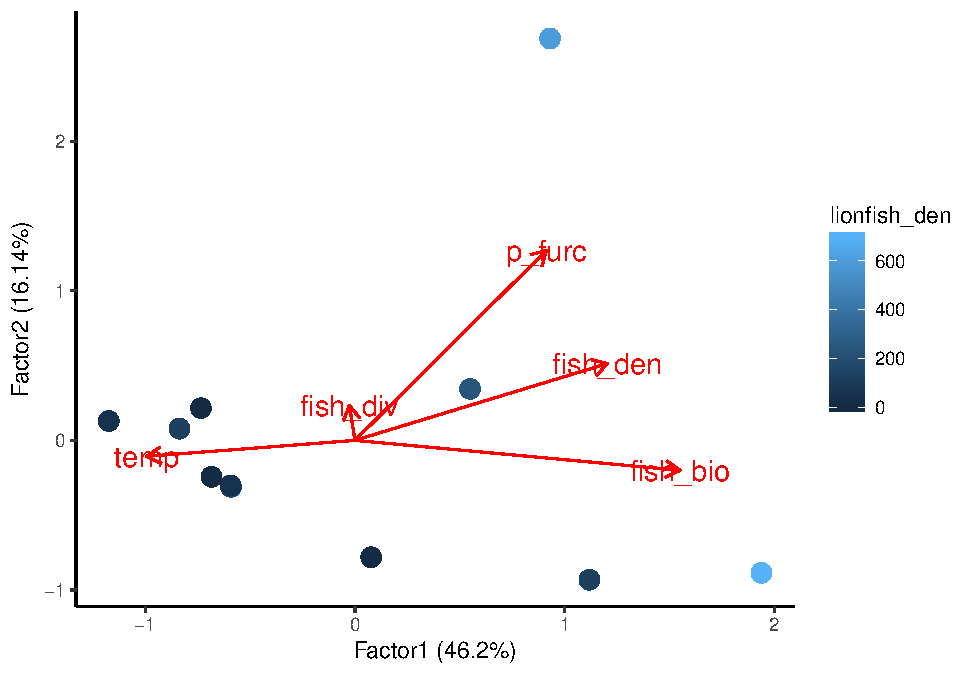
\includegraphics{darwin_GLM_final_files/figure-latex/unnamed-chunk-7-1.pdf}

NOW FOR THE GLM \emph{using Gamma distribution as this model results in
the most ``normal'' data, see plots below of model fits}

\begin{Shaded}
\begin{Highlighting}[]
\KeywordTok{scale}\NormalTok{((darwin[,}\DecValTok{2}\OperatorTok{:}\DecValTok{8}\NormalTok{]), }\DataTypeTok{center =} \OtherTok{TRUE}\NormalTok{, }\DataTypeTok{scale =} \OtherTok{TRUE}\NormalTok{)}
\end{Highlighting}
\end{Shaded}

\begin{verbatim}
##         fish_div   fish_den   fish_bio        temp       c_bda    c_enchry
##  [1,]  0.4809800  1.4365108  1.2281635 -0.09399786  0.09054847  2.60244718
##  [2,] -0.0497952  2.0336000  0.5682290 -0.78331818  0.23309789 -0.43401594
##  [3,] -0.1564501  0.8528393  2.0426555 -1.47263851 -0.37682665  0.99732680
##  [4,]  0.2879963 -0.6834913  0.5114883 -0.09399786 -0.73904237  0.08487951
##  [5,] -0.5657100 -0.7103267 -0.5480014 -0.09399786 -0.57546108 -0.64805727
##  [6,]  0.0724305 -0.7639977 -0.8468391 -1.12797821 -0.59882984 -0.48007135
##  [7,]  0.2267893  0.0410664 -0.5568844 -0.09399786  2.35211988 -0.66488296
##  [8,] -1.3837317 -0.1199464  0.1806320  0.59532246  1.36414569 -0.65962493
##  [9,] -0.7697882 -0.6029849 -0.6502334 -0.09399786 -0.73904237  0.10444226
## [10,]  2.5176680 -0.6029849 -0.7515916  1.28463865 -0.27166725 -0.23756036
## [11,] -0.6603889 -0.8802847 -1.1776184  1.97396311 -0.73904237 -0.66488296
##           p_furc
##  [1,] -0.1154827
##  [2,]  2.7300946
##  [3,]  0.4089936
##  [4,]  0.6103919
##  [5,] -0.5969805
##  [6,] -0.4244987
##  [7,] -0.5969805
##  [8,] -0.5908870
##  [9,] -0.5969805
## [10,] -0.2520169
## [11,] -0.5756534
## attr(,"scaled:center")
##     fish_div     fish_den     fish_bio         temp        c_bda 
## 1.043875e+00 3.456499e+03 2.160150e+05 2.229798e+01 7.658861e+03 
##     c_enchry       p_furc 
## 5.930354e+04 2.953466e+04 
## attr(,"scaled:scale")
##     fish_div     fish_den     fish_bio         temp        c_bda 
## 2.459291e-01 3.105964e+03 1.395158e+05 8.059469e-01 1.036322e+04 
##     c_enchry       p_furc 
## 8.919395e+04 4.947341e+04
\end{verbatim}

\begin{Shaded}
\begin{Highlighting}[]
\NormalTok{fit_bio <-}\StringTok{ }\KeywordTok{glm}\NormalTok{((lionfish_den }\OperatorTok{+}\StringTok{ }\DecValTok{1}\NormalTok{)}\OperatorTok{~}\NormalTok{fish_bio, }\DataTypeTok{data=}\NormalTok{darwin, }\DataTypeTok{family =}\NormalTok{ Gamma)}
\NormalTok{fit_den <-}\StringTok{ }\KeywordTok{glm}\NormalTok{((lionfish_den }\OperatorTok{+}\StringTok{ }\DecValTok{1}\NormalTok{)}\OperatorTok{~}\NormalTok{fish_den, }\DataTypeTok{data=}\NormalTok{darwin, }\DataTypeTok{family =}\NormalTok{ Gamma)}
\NormalTok{fit_div <-}\StringTok{ }\KeywordTok{glm}\NormalTok{((lionfish_den }\OperatorTok{+}\StringTok{ }\DecValTok{1}\NormalTok{)}\OperatorTok{~}\NormalTok{fish_div, }\DataTypeTok{data=}\NormalTok{darwin,}\DataTypeTok{family =}\NormalTok{ Gamma, }\DataTypeTok{start =} \KeywordTok{c}\NormalTok{(}\FloatTok{0.5}\NormalTok{, }\FloatTok{0.5}\NormalTok{))}
\end{Highlighting}
\end{Shaded}

\begin{verbatim}
## Warning in log(ifelse(y == 0, 1, y/mu)): NaNs produced
\end{verbatim}

\begin{verbatim}
## Warning: step size truncated due to divergence
\end{verbatim}

\begin{verbatim}
## Warning in log(ifelse(y == 0, 1, y/mu)): NaNs produced

## Warning in log(ifelse(y == 0, 1, y/mu)): NaNs produced

## Warning in log(ifelse(y == 0, 1, y/mu)): NaNs produced

## Warning in log(ifelse(y == 0, 1, y/mu)): NaNs produced

## Warning in log(ifelse(y == 0, 1, y/mu)): NaNs produced

## Warning in log(ifelse(y == 0, 1, y/mu)): NaNs produced

## Warning in log(ifelse(y == 0, 1, y/mu)): NaNs produced

## Warning in log(ifelse(y == 0, 1, y/mu)): NaNs produced
\end{verbatim}

\begin{verbatim}
## Warning: step size truncated due to divergence
\end{verbatim}

\begin{verbatim}
## Warning in log(ifelse(y == 0, 1, y/mu)): NaNs produced

## Warning in log(ifelse(y == 0, 1, y/mu)): NaNs produced

## Warning in log(ifelse(y == 0, 1, y/mu)): NaNs produced

## Warning in log(ifelse(y == 0, 1, y/mu)): NaNs produced

## Warning in log(ifelse(y == 0, 1, y/mu)): NaNs produced

## Warning in log(ifelse(y == 0, 1, y/mu)): NaNs produced
\end{verbatim}

\begin{verbatim}
## Warning: step size truncated due to divergence
\end{verbatim}

\begin{verbatim}
## Warning in log(ifelse(y == 0, 1, y/mu)): NaNs produced

## Warning in log(ifelse(y == 0, 1, y/mu)): NaNs produced

## Warning in log(ifelse(y == 0, 1, y/mu)): NaNs produced

## Warning in log(ifelse(y == 0, 1, y/mu)): NaNs produced
\end{verbatim}

\begin{verbatim}
## Warning: step size truncated due to divergence
\end{verbatim}

\begin{verbatim}
## Warning in log(ifelse(y == 0, 1, y/mu)): NaNs produced
\end{verbatim}

\begin{Shaded}
\begin{Highlighting}[]
\NormalTok{fit_pfur <-}\StringTok{ }\KeywordTok{glm}\NormalTok{((lionfish_den }\OperatorTok{+}\StringTok{ }\DecValTok{1}\NormalTok{)}\OperatorTok{~}\NormalTok{p_furc, }\DataTypeTok{data=}\NormalTok{darwin,}\DataTypeTok{family =}\NormalTok{ Gamma)}
\NormalTok{fit_temp <-}\StringTok{ }\KeywordTok{glm}\NormalTok{((lionfish_den }\OperatorTok{+}\StringTok{ }\DecValTok{1}\NormalTok{)}\OperatorTok{~}\NormalTok{temp, }\DataTypeTok{data=}\NormalTok{darwin, }\DataTypeTok{family =}\NormalTok{ Gamma)}
\KeywordTok{AIC}\NormalTok{(fit_bio, fit_den, fit_pfur, fit_temp, fit_div)}
\end{Highlighting}
\end{Shaded}

\begin{verbatim}
##          df      AIC
## fit_bio   3 132.1325
## fit_den   3 132.9021
## fit_pfur  3 133.0543
## fit_temp  3 130.8770
## fit_div   3 135.4520
\end{verbatim}

\begin{Shaded}
\begin{Highlighting}[]
\KeywordTok{coef}\NormalTok{(fit_bio, fit_den, fit_pfur, fit_temp, fit_div)}
\end{Highlighting}
\end{Shaded}

\begin{verbatim}
##   (Intercept)      fish_bio 
##  1.418382e-02 -2.590616e-08
\end{verbatim}

\begin{Shaded}
\begin{Highlighting}[]
\KeywordTok{summary}\NormalTok{(fit_bio)}
\end{Highlighting}
\end{Shaded}

\begin{verbatim}
## 
## Call:
## glm(formula = (lionfish_den + 1) ~ fish_bio, family = Gamma, 
##     data = darwin)
## 
## Deviance Residuals: 
##     Min       1Q   Median       3Q      Max  
## -2.7729  -1.6877  -0.5795   0.4458   1.7658  
## 
## Coefficients:
##               Estimate Std. Error t value Pr(>|t|)  
## (Intercept)  1.418e-02  5.939e-03   2.388   0.0407 *
## fish_bio    -2.591e-08  1.270e-08  -2.039   0.0718 .
## ---
## Signif. codes:  0 '***' 0.001 '**' 0.01 '*' 0.05 '.' 0.1 ' ' 1
## 
## (Dispersion parameter for Gamma family taken to be 1.485765)
## 
##     Null deviance: 33.732  on 10  degrees of freedom
## Residual deviance: 26.879  on  9  degrees of freedom
## AIC: 132.13
## 
## Number of Fisher Scoring iterations: 7
\end{verbatim}

\begin{Shaded}
\begin{Highlighting}[]
\KeywordTok{summary}\NormalTok{(fit_den)}
\end{Highlighting}
\end{Shaded}

\begin{verbatim}
## 
## Call:
## glm(formula = (lionfish_den + 1) ~ fish_den, family = Gamma, 
##     data = darwin)
## 
## Deviance Residuals: 
##     Min       1Q   Median       3Q      Max  
## -2.7576  -1.8288  -0.7249   0.3836   1.6406  
## 
## Coefficients:
##               Estimate Std. Error t value Pr(>|t|)  
## (Intercept)  1.144e-02  4.857e-03   2.355   0.0430 *
## fish_den    -1.024e-06  5.547e-07  -1.845   0.0981 .
## ---
## Signif. codes:  0 '***' 0.001 '**' 0.01 '*' 0.05 '.' 0.1 ' ' 1
## 
## (Dispersion parameter for Gamma family taken to be 1.50623)
## 
##     Null deviance: 33.732  on 10  degrees of freedom
## Residual deviance: 28.346  on  9  degrees of freedom
## AIC: 132.9
## 
## Number of Fisher Scoring iterations: 7
\end{verbatim}

\begin{Shaded}
\begin{Highlighting}[]
\KeywordTok{summary}\NormalTok{(fit_div)}
\end{Highlighting}
\end{Shaded}

\begin{verbatim}
## 
## Call:
## glm(formula = (lionfish_den + 1) ~ fish_div, family = Gamma, 
##     data = darwin, start = c(0.5, 0.5))
## 
## Deviance Residuals: 
##      Min        1Q    Median        3Q       Max  
## -2.93731  -2.04226  -0.38759   0.06849   1.69945  
## 
## Coefficients:
##             Estimate Std. Error t value Pr(>|t|)
## (Intercept) 0.003937   0.010800   0.365    0.724
## fish_div    0.001435   0.010377   0.138    0.893
## 
## (Dispersion parameter for Gamma family taken to be 1.923602)
## 
##     Null deviance: 33.732  on 10  degrees of freedom
## Residual deviance: 33.694  on  9  degrees of freedom
## AIC: 135.45
## 
## Number of Fisher Scoring iterations: 8
\end{verbatim}

\begin{Shaded}
\begin{Highlighting}[]
\KeywordTok{summary}\NormalTok{(fit_pfur)}
\end{Highlighting}
\end{Shaded}

\begin{verbatim}
## 
## Call:
## glm(formula = (lionfish_den + 1) ~ p_furc, family = Gamma, data = darwin)
## 
## Deviance Residuals: 
##     Min       1Q   Median       3Q      Max  
## -2.7662  -1.8014  -0.2507   0.2023   2.0405  
## 
## Coefficients:
##               Estimate Std. Error t value Pr(>|t|)  
## (Intercept)  8.872e-03  3.963e-03   2.239   0.0519 .
## p_furc      -4.612e-08  2.690e-08  -1.714   0.1206  
## ---
## Signif. codes:  0 '***' 0.001 '**' 0.01 '*' 0.05 '.' 0.1 ' ' 1
## 
## (Dispersion parameter for Gamma family taken to be 1.917667)
## 
##     Null deviance: 33.732  on 10  degrees of freedom
## Residual deviance: 28.644  on  9  degrees of freedom
## AIC: 133.05
## 
## Number of Fisher Scoring iterations: 7
\end{verbatim}

\begin{Shaded}
\begin{Highlighting}[]
\KeywordTok{summary}\NormalTok{(fit_temp)}
\end{Highlighting}
\end{Shaded}

\begin{verbatim}
## 
## Call:
## glm(formula = (lionfish_den + 1) ~ temp, family = Gamma, data = darwin)
## 
## Deviance Residuals: 
##     Min       1Q   Median       3Q      Max  
## -2.6965  -1.6239  -0.2054   0.3340   1.4827  
## 
## Coefficients:
##              Estimate Std. Error t value Pr(>|t|)  
## (Intercept) -0.163059   0.071533  -2.279   0.0486 *
## temp         0.007778   0.003367   2.310   0.0462 *
## ---
## Signif. codes:  0 '***' 0.001 '**' 0.01 '*' 0.05 '.' 0.1 ' ' 1
## 
## (Dispersion parameter for Gamma family taken to be 1.237724)
## 
##     Null deviance: 33.732  on 10  degrees of freedom
## Residual deviance: 24.624  on  9  degrees of freedom
## AIC: 130.88
## 
## Number of Fisher Scoring iterations: 6
\end{verbatim}

\begin{Shaded}
\begin{Highlighting}[]
\KeywordTok{hist}\NormalTok{(}\KeywordTok{resid}\NormalTok{(fit_temp))}
\end{Highlighting}
\end{Shaded}

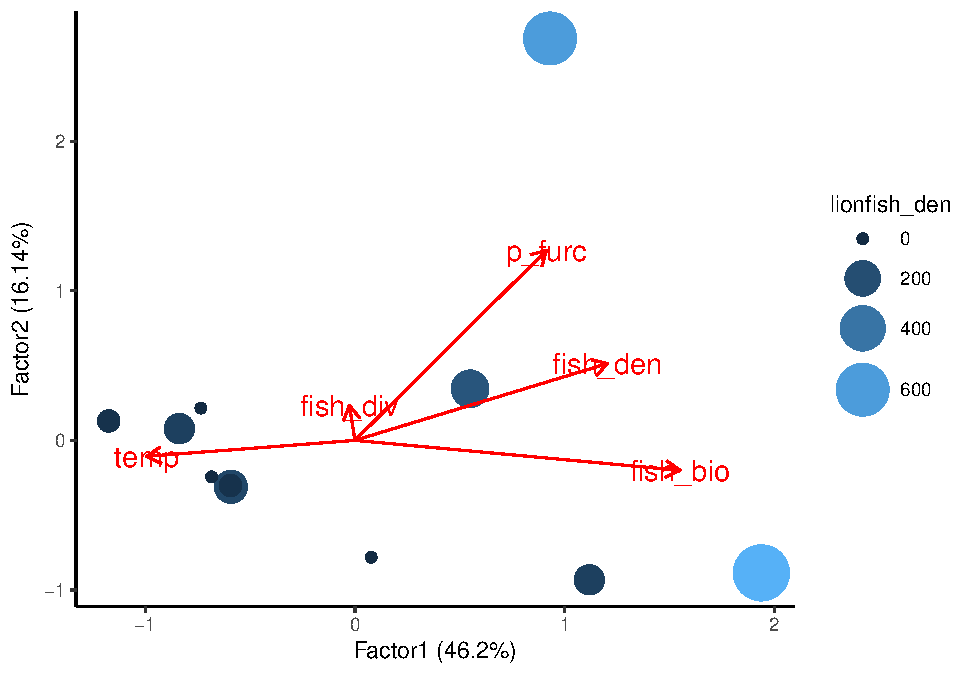
\includegraphics{darwin_GLM_final_files/figure-latex/unnamed-chunk-9-1.pdf}

\begin{Shaded}
\begin{Highlighting}[]
\KeywordTok{qqnorm}\NormalTok{(}\KeywordTok{resid}\NormalTok{(fit_temp))}
\KeywordTok{qqline}\NormalTok{(}\KeywordTok{resid}\NormalTok{(fit_temp))}
\end{Highlighting}
\end{Shaded}

\includegraphics{darwin_GLM_final_files/figure-latex/unnamed-chunk-9-2.pdf}

\begin{Shaded}
\begin{Highlighting}[]
\KeywordTok{hist}\NormalTok{(}\KeywordTok{resid}\NormalTok{(fit_den))}
\end{Highlighting}
\end{Shaded}

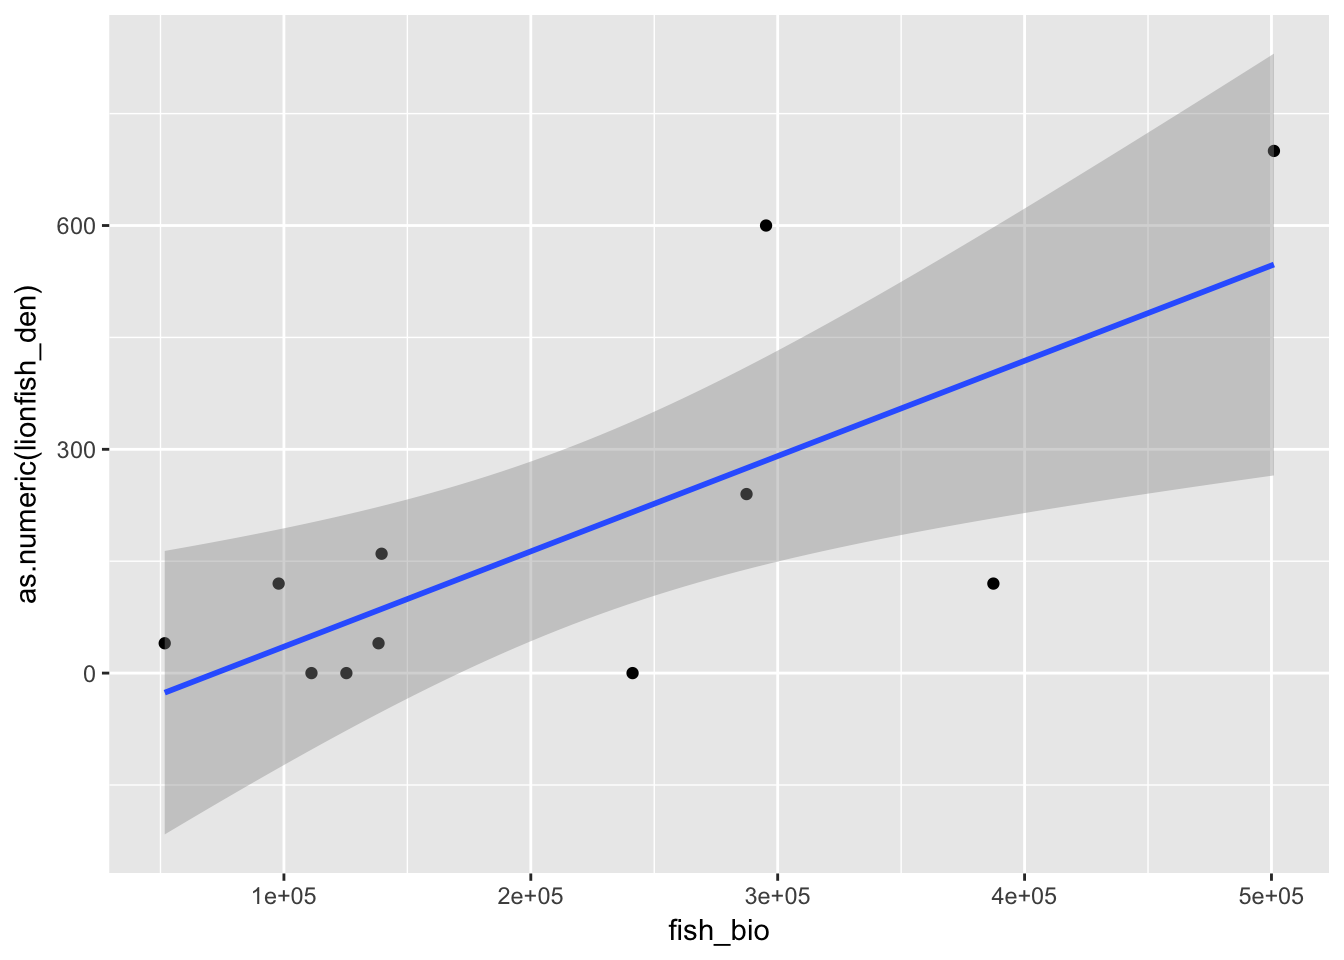
\includegraphics{darwin_GLM_final_files/figure-latex/unnamed-chunk-10-1.pdf}

\begin{Shaded}
\begin{Highlighting}[]
\KeywordTok{qqnorm}\NormalTok{(}\KeywordTok{resid}\NormalTok{(fit_den))}
\KeywordTok{qqline}\NormalTok{(}\KeywordTok{resid}\NormalTok{(fit_den))}
\end{Highlighting}
\end{Shaded}

\includegraphics{darwin_GLM_final_files/figure-latex/unnamed-chunk-10-2.pdf}

\begin{Shaded}
\begin{Highlighting}[]
\KeywordTok{hist}\NormalTok{(}\KeywordTok{resid}\NormalTok{(fit_div))}
\end{Highlighting}
\end{Shaded}

\includegraphics{darwin_GLM_final_files/figure-latex/unnamed-chunk-11-1.pdf}

\begin{Shaded}
\begin{Highlighting}[]
\KeywordTok{qqnorm}\NormalTok{(}\KeywordTok{resid}\NormalTok{(fit_div))}
\KeywordTok{qqline}\NormalTok{(}\KeywordTok{resid}\NormalTok{(fit_div))}
\end{Highlighting}
\end{Shaded}

\includegraphics{darwin_GLM_final_files/figure-latex/unnamed-chunk-11-2.pdf}

\begin{Shaded}
\begin{Highlighting}[]
\KeywordTok{hist}\NormalTok{(}\KeywordTok{resid}\NormalTok{(fit_bio))}
\end{Highlighting}
\end{Shaded}

\includegraphics{darwin_GLM_final_files/figure-latex/unnamed-chunk-12-1.pdf}

\begin{Shaded}
\begin{Highlighting}[]
\KeywordTok{qqnorm}\NormalTok{(}\KeywordTok{resid}\NormalTok{(fit_bio))}
\KeywordTok{qqline}\NormalTok{(}\KeywordTok{resid}\NormalTok{(fit_bio))}
\end{Highlighting}
\end{Shaded}

\includegraphics{darwin_GLM_final_files/figure-latex/unnamed-chunk-12-2.pdf}

\begin{Shaded}
\begin{Highlighting}[]
\KeywordTok{hist}\NormalTok{(}\KeywordTok{resid}\NormalTok{(fit_pfur))}
\end{Highlighting}
\end{Shaded}

\includegraphics{darwin_GLM_final_files/figure-latex/unnamed-chunk-13-1.pdf}

\begin{Shaded}
\begin{Highlighting}[]
\KeywordTok{qqnorm}\NormalTok{(}\KeywordTok{resid}\NormalTok{(fit_pfur))}
\KeywordTok{qqline}\NormalTok{(}\KeywordTok{resid}\NormalTok{(fit_pfur))}
\end{Highlighting}
\end{Shaded}

\includegraphics{darwin_GLM_final_files/figure-latex/unnamed-chunk-13-2.pdf}

\begin{Shaded}
\begin{Highlighting}[]
\KeywordTok{coef}\NormalTok{(fit_bio)}
\end{Highlighting}
\end{Shaded}

\begin{verbatim}
##   (Intercept)      fish_bio 
##  1.418382e-02 -2.590616e-08
\end{verbatim}

\begin{Shaded}
\begin{Highlighting}[]
\KeywordTok{coef}\NormalTok{(fit_pfur) }
\end{Highlighting}
\end{Shaded}

\begin{verbatim}
##   (Intercept)        p_furc 
##  8.871575e-03 -4.611608e-08
\end{verbatim}

\begin{Shaded}
\begin{Highlighting}[]
\KeywordTok{coef}\NormalTok{(fit_temp) }
\end{Highlighting}
\end{Shaded}

\begin{verbatim}
##  (Intercept)         temp 
## -0.163058692  0.007778458
\end{verbatim}

\begin{Shaded}
\begin{Highlighting}[]
\KeywordTok{coef}\NormalTok{(fit_div)}
\end{Highlighting}
\end{Shaded}

\begin{verbatim}
## (Intercept)    fish_div 
## 0.003937398 0.001435102
\end{verbatim}

\begin{Shaded}
\begin{Highlighting}[]
\KeywordTok{coef}\NormalTok{(fit_den)}
\end{Highlighting}
\end{Shaded}

\begin{verbatim}
##   (Intercept)      fish_den 
##  1.143692e-02 -1.023463e-06
\end{verbatim}


\end{document}
